% \documentclass[PhD]{iitmdiss}
%\documentclass[MS]{iitmdiss}
\documentclass[MTech]{iitmdiss}
\documentclass[BTech]{iitmdiss}
\usepackage{times}
 \usepackage{t1enc}
 \usepackage[usenames,dvipsnames,svgnames,table]{xcolor}
\usepackage{amsmath, amssymb}
\usepackage{mathtools}
\usepackage{caption}
\usepackage{algorithm}
\usepackage[noend]{algpseudocode}
\usepackage{graphicx}
\usepackage{epstopdf}
\usepackage{multirow}% http://ctan.org/pkg/multirow
\usepackage{hhline}%
\usepackage{listings}
\setcounter{secnumdepth}{5}
\usepackage[hypertex]{hyperref} % hyperlinks for references.
\graphicspath{{Images/}}

\begin{document}


%%%%%%%%%%%%%%%%%%%%%%%%%%%%%%%%%%%%%%%%%%%%%%%%%%%%%%%%%%%%%%%%%%%%%%
% Title page
\definecolor{lbcolor}{rgb}{0.9,0.9,0.9}
\lstset{
    %frame=tb, % draw a frame at the top and bottom of the code block
    backgroundcolor=\color{lbcolor},
    tabsize=4, % tab space width
    showstringspaces=false, % don't mark spaces in strings
    %numbers=left, % display line numbers on the left
    commentstyle=\color{green}, % comment color
    keywordstyle=\color{blue}, % keyword color
    stringstyle=\color{red}, % string color
    breaklines=true,
}
\title{Concurrent AVL Tree Operations on GPUs}

\author{Abhishek Yadav}

\date{APRIL 2017}
\department{COMPUTER SCIENCE AND EGNINEERING}
\newcolumntype{C}[1]{>{\centering}m{#1}}
%\nocite{*}
\maketitle

%%%%%%%%%%%%%%%%%%%%%%%%%%%%%%%%%%%%%%%%%%%%%%%%%%%%%%%%%%%%%%%%%%%%%%
% Certificate
\certificate

\vspace*{0.5in}

\noindent This is to certify that the thesis titled {\bf Concurrent AVL Tree Operations on GPUs}, submitted by {\bf Abhishek Yadav}, 
  to the Indian Institute of Technology, Madras, for
the award of the degree of {\bf B.Tech + M.Tech}, is a bona fide
record of the research work done by him under our supervision.  The
contents of this thesis, in full or in parts, have not been submitted
to any other Institute or University for the award of any degree or
diploma.

\vspace*{1.5in}

\begin{singlespacing}
\hspace*{-0.25in}
\parbox{2.5in}{
\noindent {\bf Dr. Rupesh Nasre} \\
\noindent Research Guide \\ 
\noindent Professor \\
\noindent Dept. of Computer Science and Engineering\\
\noindent IIT-Madras, 600 036 \\
} 
\hspace*{1.0in} 
%\parbox{2.5in}{
%\noindent {\bf Prof.~S.~C.~Rajan} \\
%\noindent Research Guide \\ 
%\noindent Assistant Professor \\
%\noindent Dept.  of  Aerospace Engineering\\
%\noindent IIT-Madras, 600 036 \\
%}  
\end{singlespacing}
\vspace*{0.25in}
\noindent Place: Chennai\\
Date: 10th March 2017 


%%%%%%%%%%%%%%%%%%%%%%%%%%%%%%%%%%%%%%%%%%%%%%%%%%%%%%%%%%%%%%%%%%%%%%
% Acknowledgements
\acknowledgements
I am very thankful to my advisor \textbf{Dr. Rupesh Nasre} for letting me work with him on this project and guiding me through the completion of it. He has been kind enough to let me switch the implementation framework from \textbf{OpenCl} to \textbf{Cuda} owing to lack of proper documentation and online support available for the former. He has been quite encouraging and helped me through his suggestions and invaluable inputs for the project.  

\indent I am indebted to IIT Madras and Department of Computer Science and Engineering for providing me the opportunities I never imagined and being the place of best of the times of my life. I would like to thank my friends and professors for their support throughout without whom I wouldn't be the person I am.       
%%%%%%%%%%%%%%%%%%%%%%%%%%%%%%%%%%%%%%%%%%%%%%%%%%%%%%%%%%%%%%%%%%%%%%
% Abstract

\abstract

\vspace*{24pt}

\noindent
Recent developments in GPU architecture has prompted researchers to use GPUs to improve the performance of the algorithms which can be parallelized. Several algorithms to perform concurrent insertions, deletions and searches on AVL Tree have been published. However, these algorithms have been implemented to run on multicore CPUs which are optimized for sequential execution and can launch very few number of threads as compared to GPUs. Since general purpose GPUs consist thousands of smaller cores optimized for
parallel processing these can be used to execute parallel tasks over multi-core CPUs. Update operations are bottlenecks in the performance of AVL trees in concurrent environment. My work is inspired from the work in \cite{Logical_Ordering} which introduces the novel concept of Logical Ordering of the tree elements in order to perform concurrent lock-free searches along with update operations. 


\pagebreak

%%%%%%%%%%%%%%%%%%%%%%%%%%%%%%%%%%%%%%%%%%%%%%%%%%%%%%%%%%%%%%%%%
% Table of contents etc.

\begin{singlespace}
\tableofcontents
\end{singlespace}

\clearpage

% The main text will follow from this point so set the page numbering
% to arabic from here on.
\pagenumbering{arabic}


%%%%%%%%%%%%%%%%%%%%%%%%%%%%%%%%%%%%%%%%%%%%%%%%%%
% Introduction.

\chapter{INTRODUCTION}
\label{chap:intro}

\section{Binary Search Trees}
Binary Search Trees are excellent data structures to implement maps, databases, symbol tables, sets and similar such interfaces. But they are efficient only when they are balanced because straightforward insertions, in the worst case, can lead to highly unbalanced trees which will result in inefficient search(which is required for both deletion and insertion operations) complexity.  The solution to this problem is to dynamically rebalance the tree during insert/search/delete operations without
destroying the ordering invariant. These type of self-balancing binary search trees have some property which must hold for each node after every operation. Self-balancing property of Balanced Binary Search Trees restrains their heights to O(\(\log(n)\)) which results in efficient height-dependent tree operations and thereby making such structures desirable for applications which require efficient access to their data. 


\section{AVL Trees}
AVL Tree, named named after its inventors Adel'son-Vel'skii and Landis is balanced binary search tree. AVL trees maintain \textit{height invariant} property which means, for any internal node, the heights of its left and right subtrees can differ by at most
one. After insert and delete operations, \textit{height invariant} property may not hold for some nodes and thus requires rebalancing operations to be performed to restore the height-invariant property of the tree. For the convenience of representation, we define left child, right child, height and parent of a node n as \textbf{left}(n),
\textbf{right}(n), \textbf{height}(n) and \textbf{parent}(n) respectively. Some more notations will be introduced later to represent certain properties of
the nodes during concurrent operations. Height of any node, n, is defined as:
\[
	\textbf{height}(n) = 
	\begin{cases*}
		-1, & \text{if n=NULL}\\
        1+\textbf{max}(\textbf{height}(\textbf{left}(n)), \textbf{height}(\textbf{right}(n)), & otherwise 
    \end{cases*}
\]


\textit{Balance factor}, \textbf{bal}(n) of a node n, is defined as the difference in heights of the subtrees rooted at n. Some authors define it as \textbf{bal}(n) = \textbf{height}(\textbf{left}(n)) - \textbf{height}(\textbf{right}(n)) whereas others define it as \textbf{bal}(n) = \textbf{height}(\textbf{right}(n)) - \textbf{height}(\textbf{left}(n)).
I have used the first definition of balance factor throughout. Thus, a Binary Search Tree is an AVL tree if, for each node,n, of the tree, \textbf{bal}(n) $\in\{-1,0,1\}$. 


\section{AVL Tree Rotations}
In an AVL tree, after performing insertion and deletion operations heights of the nodes in the path of insertion/deletion gets changed. Consequently, the \textbf{balance factor} of some of the nodes on the path of insertion/deletion also gets changed. If
all the nodes on the path of insertion/deletion satisfy the balance factor condition then operations conclude the same way as in typical binary search tree otherwise rotation operations are performed on one or more nodes to maintain the height invariant
or balance factor of the tree. We define critical node, \textbf{cn} as the node in the path of insertion/deletion whose balance factor may not satisfy the balance-factor invariant of the avl tree. If balance factor of the critical node does not satisfy the balance-factor property of the avl tree, depending on the direction of insertion/deletion w.r.t. critical node, one of the following four rotation
operations are performed to maintain the balance-factor invariant of the affected nodes:

\subsection{Single Left Rotation}
If a node is inserted to the right of the right child of the critical node, \textbf{cn}, resulting in the violation of height-invariant property of \textbf{cn}, a single \textbf{left-rotation} is used to balance the tree. Let t=\textbf{right}(cn), following changes take place as a result of the rotation-
\begin{itemize}
    \item \textbf{parent}(t) $\leftarrow$ \textbf{parent}(cn)
    \item \textbf{parent}(cn) $\leftarrow$ t
    \item \textbf{right}(cn) $\leftarrow$ \textbf{left}(t)
    \item \textbf{parent}(\textbf{left}(t)) $\leftarrow$ cn
    \item \textbf{left}(t) = cn
    \item  \textbf{left}(\textbf{parent}(t)) $\leftarrow$ t or \textbf{right}(\textbf{parent}(t)) $\leftarrow$ t  depending on whether cn was the left or the right child of its parent.
\end{itemize}
Heights of \textbf{cn}, \textbf{t} and \textbf{parent}(t) are updated based on the heights of the subtrees added to the left/right of them. 
In figure \ref{fig:single_left}, node \textbf{a} is a critical node whose \textbf{balance-factor} property is destroyed by an insertion in the right-subtree of its right-child \textbf{b} which is restored by a single left rotation at \textbf{a}.

\begin{figure}
\centering
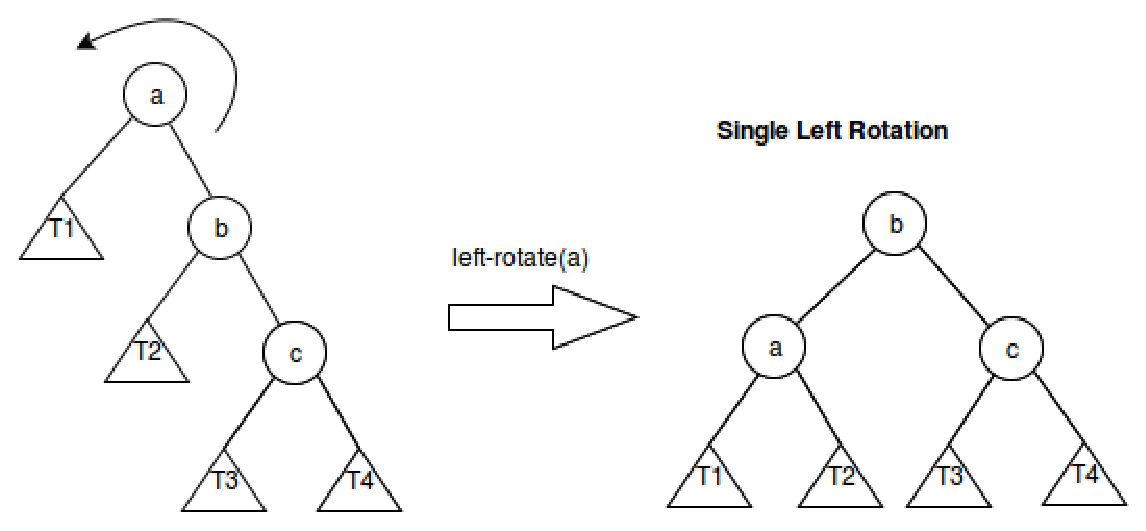
\includegraphics[width=12cm,height=5cm]{Single_Left}
\centering
\caption{Single Left Rotation}
\label{fig:single_left}
\end{figure} 

\subsection{Single Right Rotation}
If a node is inserted to the left of the left child of the critical node,\textbf{cn}, a single right-rotation at \textbf{cn} balances the tree. Let t= \textbf{left}(cn) and p=\textbf{parent}(cn), following changes take place due to rotation at \textbf{cn}-
\begin{itemize}
\item \textbf{parent}(t) $\leftarrow$ \textbf{parent}(cn)
\item \textbf{parent}(cn) $\leftarrow$ t
\item \textbf{left}(cn) $\leftarrow$ \textbf{right}(t)
\item \textbf{parent}(\textbf{right}(t)) $\leftarrow$ cn
\item \textbf{right}(t) = cn
\end{itemize}
Assuming that the \textbf{cn} was the left-child of its parent before rotation, heights of the nodes affected after this rotation are updated as follows:
\begin{align*}
	\textbf{height}(cn) &= 1 + \max(\textbf{height}(\textbf{left}(cn)),\textbf{height}(\textbf{right}(cn)))\\
    \textbf{height}(t) &= 1 + \max(\textbf{height}(cn), \textbf{height}(\textbf{left}(t)))\\
    \textbf{height}(p) &= 1 + \max(\textbf{height}(t), \textbf{height}(\textbf{right}(p)))
\end{align*}
In Fig. \ref{fig:single_right}, right rotation takes place at node \textbf{a} which is the critical node. 


% needed in second column of first page if using \IEEEpubid
%\IEEEpubidadjcol
\begin{figure}
\centering
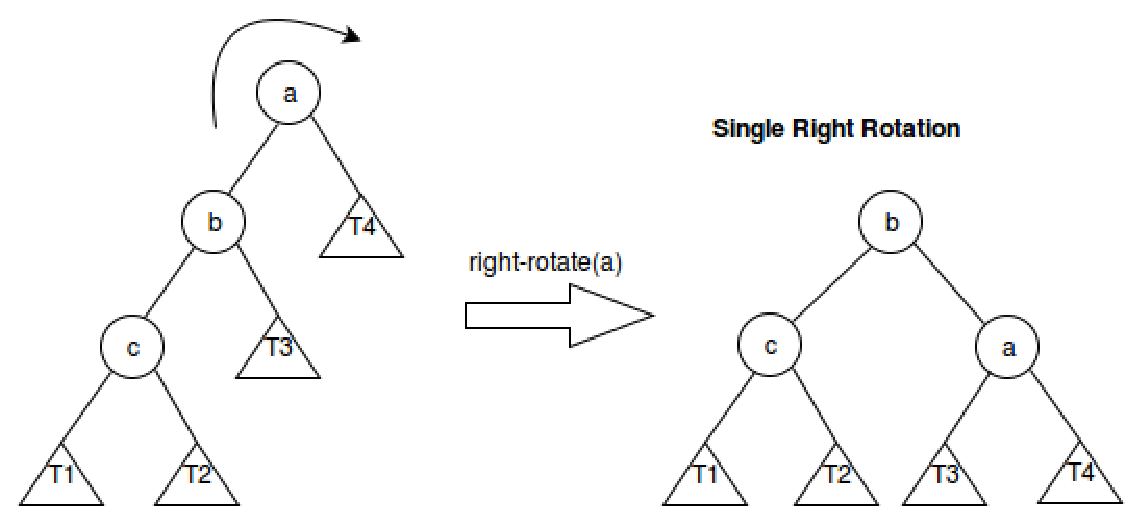
\includegraphics[width=12cm,height=5cm]{Single_Right}
\caption{Single Right Rotation}
\label{fig:single_right}
\end{figure}

\subsection*{Double Rotation - Left Right}
If the insertion of a key to the right of the left-child of the critical node, \textbf{cn}, results in the violation of height-invariant property at cn, then a double rotation is required to restore the invariant. First, a left rotation is performed at the left child of the critical node followed by a right rotation at the critical node balancing the subtree below critical node. Assuming that before rotation, parent of \textbf{cn} is p=\textbf{parent}(cn), the left child of the critical node is \textbf{l} = \textbf{left}(cn) and the right child of the \textbf{l} is \textbf{r}, following changes take place in the structure of the tree
\begin{itemize}
\item \textbf{parent}(r) $\leftarrow$ p
\item \textbf{parent}(cn)$\leftarrow$ r
\item \textbf{parent}(t) $\leftarrow$ r
\item \textbf{right}(t) $\leftarrow$ \textbf{left}(r) \hspace*{5mm} and  \textbf{parent}(\textbf{left}(r)) $\leftarrow$ t
\item \textbf{left}(cn) $\leftarrow$ \textbf{right}(r) \hspace*{5mm} and 
\textbf{parent}(\textbf{right}(r)) $\leftarrow$ cn
\item \textbf{left}(r) $\leftarrow$ t \hspace*{5mm} and \textbf{right}(r) $\leftarrow$ cn 
\end{itemize}
Depending on whether \textbf{cn} is the left or right child of \textbf{p} before rotation, \textbf{r} becomes the left or right child of \textbf{p} after rotation. Heights of \textbf{cn}, \textbf{r} and \textbf{t} are updated after rotation. Fig. \ref{fig:left_right}, shows an example of \textbf{Left Right Rotation} where a node is inserted to the right of \textbf{b} causing imbalance at critical node \textbf{a} which is fixed by a left rotation at b followed by a right rotation at \textbf{a}.   

\begin{figure}
\centering
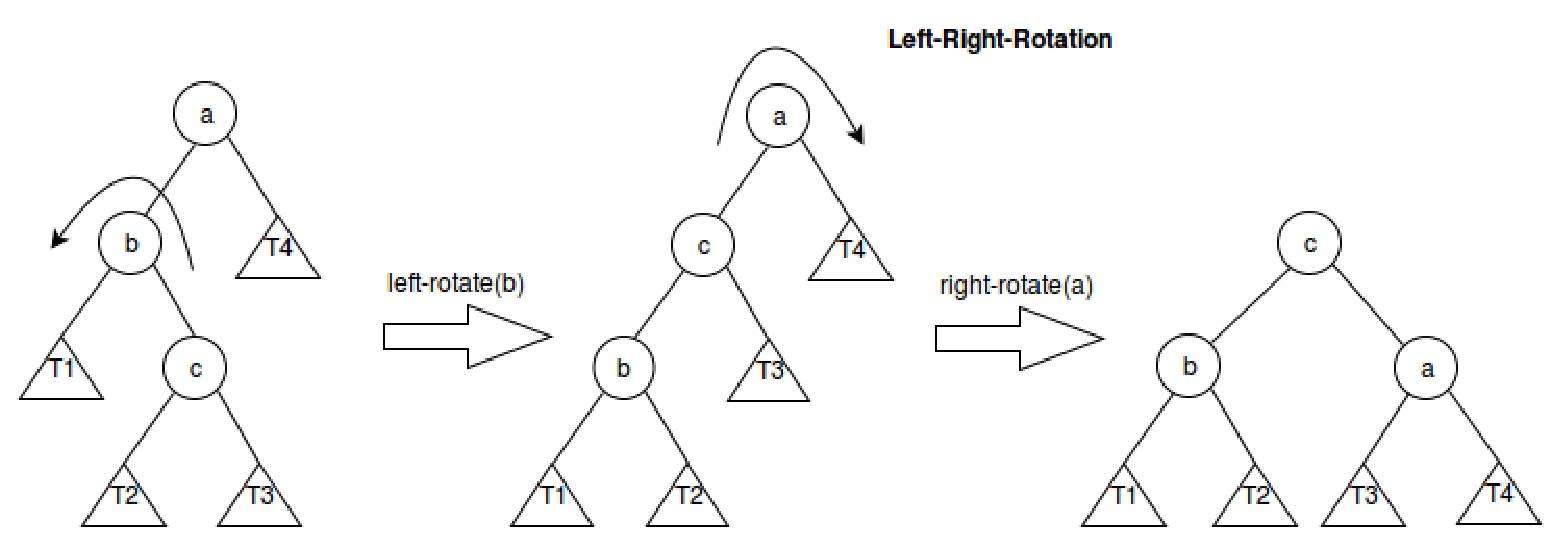
\includegraphics[width=15cm, height=5cm]{Left-Right}
\caption{Double Rotation - Left Right}
\label{fig:left_right}
\end{figure}

\subsection*{Double Rotation - Right Left}
If \textit{balance-factor} of the critical node,\textbf{cn}, gets destroyed due to insertion of a key to the left of its right child, a \textbf{double rotation - Right Left } is required to fix the \textit{balance-factor} property of the nodes in the path of insertion. In the first step of the double rotation, a \textbf{Single Right Rotation} is performed at the right child of \textbf{cn} followed by a \textit{Single Left Rotation} at \textit{cn} to fix the \textit{avl-tree-invariant} of the nodes in the insertion-path. Assuming that p=\textbf{parent}(cn), t= \textbf{right}(cn) and l=\textbf{left}(\textbf{right}(cn)) before rotation, following changes take place after double rotation - Right Left:
\begin{itemize}
\item \textbf{parent}(l) $\leftarrow$ p  and \textbf{left}(p) $\leftarrow$ l or \textbf{right}(p) $\leftarrow$ l, depending on whether \textit{cn} was the left or right child of its parent before rotation
\item \textbf{parent}(cn) $\leftarrow$ l
\item \textbf{right}(cn) $\leftarrow$ \textbf{left}(l) and \textbf{left}(l) $\leftarrow$ cn
\item \textbf{parent}(t) $\leftarrow$ l
\item \textbf{left}(t) $\leftarrow$ \textbf{right}(l) and \textbf{right}(l) $\leftarrow$ t 
\end{itemize}
Heights of the nodes \textbf{t}, \textbf{l} and \textbf{cn} are updated in after rotation. In Fig. \ref{fig:right_left}, \textbf{a} is the critical node whose balance-factor is destroyed by an insertion in the left-subtree of its right child b, Resulting in a \textit{Double Rotation - Right Left} which balances the tree by restoring the \textbf{balance-factor} property of \textbf{a,b} and \textbf{c} and makes c the parent of both a and b.

\begin{figure}
\centering
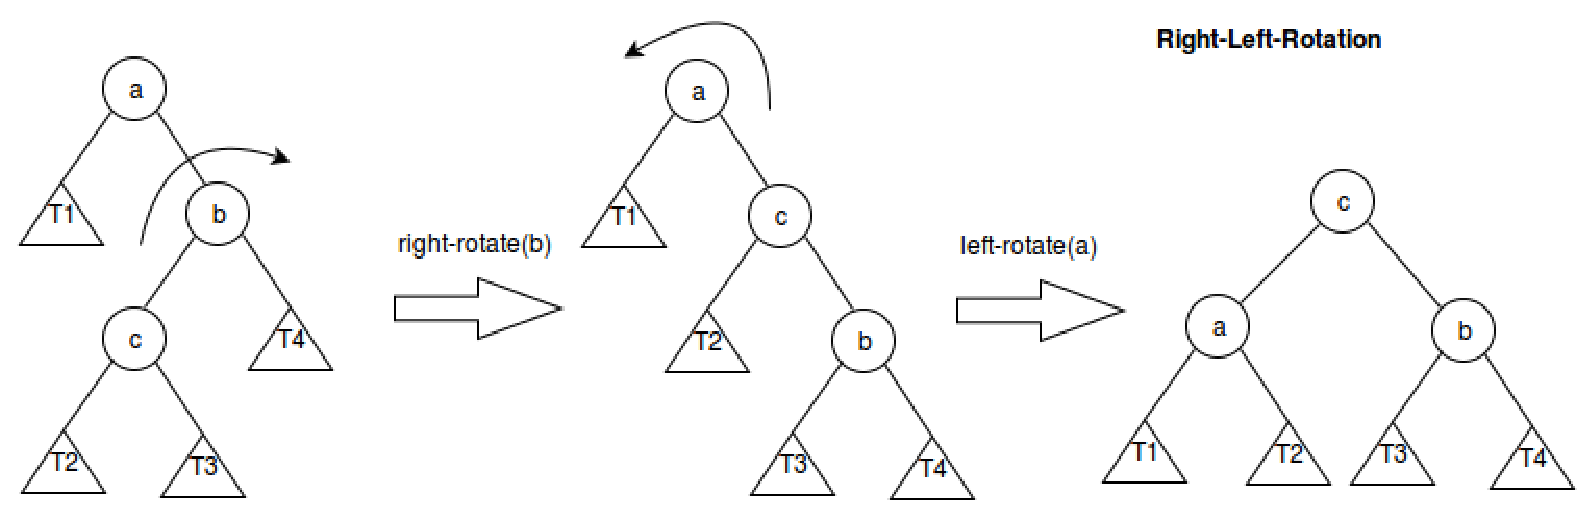
\includegraphics[width=15cm,height=5cm]{Right-Left}
\caption{Double Rotation - Right Left}
\label{fig:right_left}
\end{figure}


\section{Operations on AVL Tree}
\subsection{Search}
Search operation in AVL Tree is performed the same way as it is done in standard Binary Search Tree. Starting at root, search-key is compared with the key of each node, n, it encounters with and returns \textit{true} or n if the  \textit{search-key} matches the key of \textbf{n}, goes to the left-child of \textbf{n} if \textit{search-key} $\leq$ \textbf{key}(n) or right-child of \textbf{n} if \textit{search-key} $>$ \textbf{key}(n). If search-key is not present in the tree, it returns false or the node which would be the parent of the node containing search-key if it were to be inserted, i.e. the node where search ends without success.

%algorithm to perform search in an AVL Tree
\begin{algorithm}
\caption{Search in AVL Tree}
\begin{algorithmic}[1]
\Function{Search}{$root, key'$}
\If{$root$ == NULL}
\State \textbf{return} root
\EndIf
\State temp = $root$
\While{\textit{true}}
 \If{\textit{key}(temp) == $key'$}
 \State \textbf{return} temp
 \EndIf
 \State child = $key'$ $<$ \textbf{key}(temp) ? \textbf{left}(temp) : \textbf{right}(temp)
 \If{child == NULL}
 \State \textbf{return} temp
 \EndIf
 \State temp= child
 \EndWhile
 \EndFunction
\end{algorithmic}
\end{algorithm}


\subsection{Insertion}
First, a new node is created with the key to be inserted. If root of the tree is \textbf{null}, the  newly created node becomes the root of the tree and operation concludes, otherwise standard BST operation is performed to find the right location for the newly created node and inserts it. Next, path from newly inserted node to the root is traversed and necessary rotations are performed on the nodes whose balance factor gets disturbed as a consequence of insertion. 

\begin{algorithm}
\caption{Insertion in AVL Tree}
\begin{algorithmic}[1]
\Function{Insert}{$root,key'$}:
\State node= Search($root, key'$)
\If{node == NULL}
    \State \textbf{return} create\_node($key'$)
\ElsIf{\textit{key}(node)==$key'$}
    \State \textbf{return} node
\EndIf
\State new\_node = create\_node($key'$)
\If{\textit{key}(node) > $key'$}
\State  \textbf{left}(node) $\leftarrow$ new\_node
\Else \State \textbf{right}(node) $\leftarrow$ new\_node
\EndIf
\State \textbf{parent}(new\_node) $\leftarrow$ node
\State rebalance($root$,node,$key'$)
\EndFunction
\end{algorithmic}
\end{algorithm}


\subsection{Deletion}
Like \textit{Search} and \textit{Insert}, deletion in AVL tree is performed the same way as is done in standard Binary Search Trees. Three types of situation may arise when a node is deleted from BST which are following:
\begin{enumerate}
\item If the node to be deleted is the leaf node, as shown in Fig. \ref{fig:leaf_delete}, it is physically deleted from the tree and path from its parent to root is traversed to balance the tree.

\begin{figure}
\centering
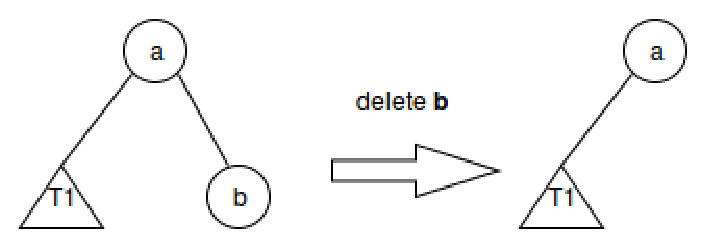
\includegraphics[width=8cm,height=2.5cm]{leaf_delete}
\caption{Deletion of a leaf node}
\label{fig:leaf_delete}
\end{figure}

\item If the node to be deleted has a single child, it is deleted physically while new links between its child and parent are formed. Parent to root path is traversed to rebalance the tree. As shown in Fig. \ref{fig:single_child_delete}, node \textbf{b} with a single child \textbf{c} is deleted and consequently c becomes the new child of \textbf{a}.

\begin{figure}
\centering 
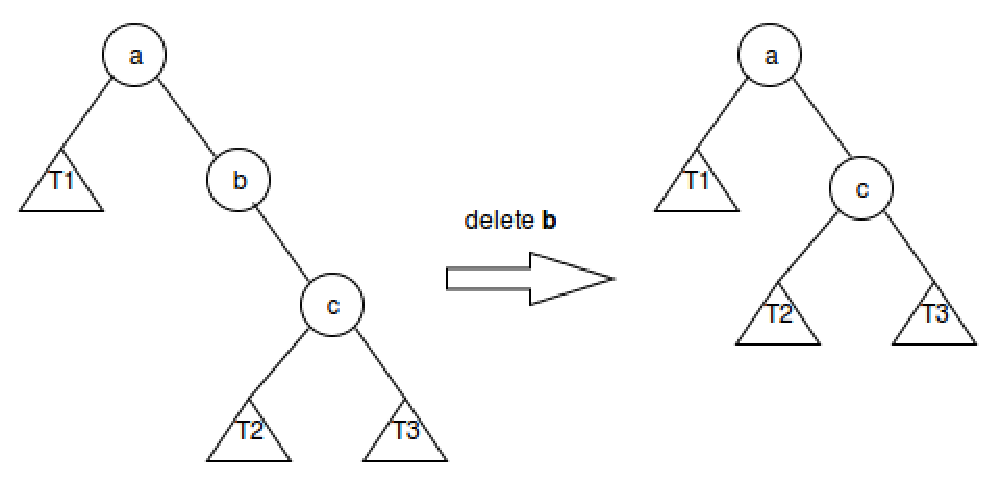
\includegraphics[width=10cm,height=5cm]{single_child_delete}
\caption{Deletion of a node with a single child}
\label{fig:single_child_delete}
\end{figure}
  
\item If the node to be deleted, \textbf{n}, has two children, first \textbf{inorder-successor} or \textbf{inorder-predecessor} of \textbf{n} is obtained (\textbf{Note:} I've considered inorder-successor in my implementation to replace the key of the node to be deleted). Next, key of \textbf{n} is replaced by the key of \textbf{succ}(n) and inorder-successor node is physically deleted. Since, inorder-successor of a node is the node with the smallest key in its right-subtree, which means that either it will have its right child or none; and hence its deletion becomes the deletion of the node with 1 or no child. As shown in Fig. \ref{fig:two_child_delete}, request to delete the node with key \textbf{b} comes which is replaced by its inorder-successor, \textbf{e} which gets physically deleted from the tree. 

\begin{figure}
\centering 
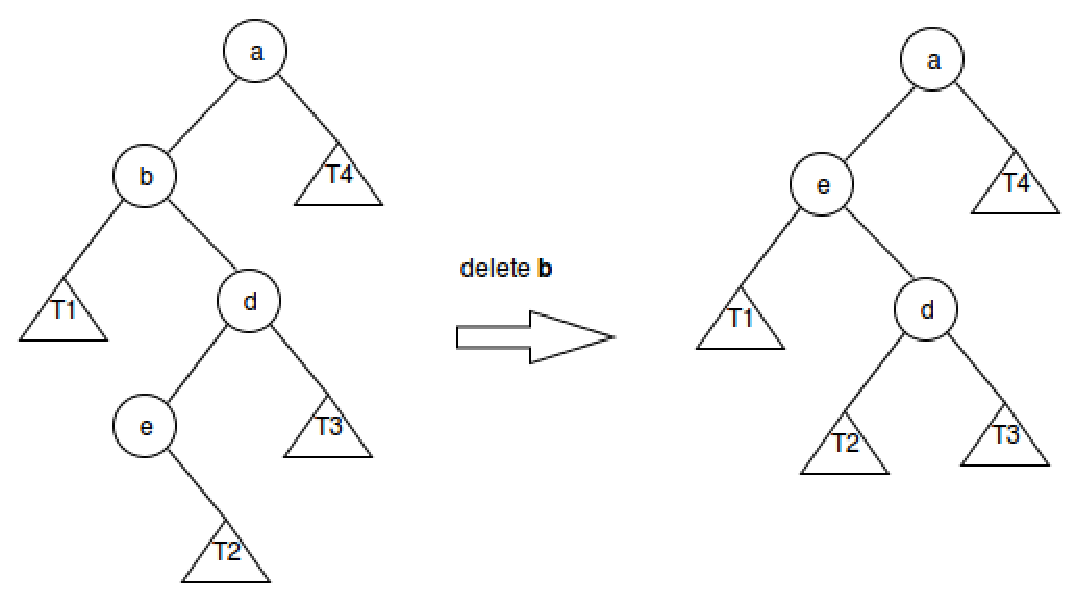
\includegraphics[width=10cm,height=6cm]{two_child_delete}
\caption{Deletion of a node with two children}
\label{fig:two_child_delete}
\end{figure}
\end{enumerate}

\begin{algorithm}
\caption{Deletion in AVL Tree}
\begin{algorithmic}[1]
\Function{delete}{$root,key'$}:
\State del\_node= search($root,key'$)
\If{del\_node == NULL}
\State \textbf{return}
\EndIf
\State p= \textbf{parent}(del\_node)
\If{\textbf{left}(del\_node) == NULL $or$ \textbf{right}(del\_node)==NULL}
	\State child= NULL
    \If{\textbf{left}(del\_node) $\neq$ NULL}
    	\State child= \textbf{left}(del\_node)
    \Else
    	\State child= \textbf{right}(del\_node)
    \EndIf
    
    \If{del\_node == \textbf{left}(p)}
    	\State \textbf{left}(p) = child
    \Else
    	\State \textbf{right}(p) = child
    \EndIf
    
    \If{child $\neq$ NULL}
    	\State \textbf{parent}(child)= p
    \EndIf
    \textbf{rebalance}($root$,p)
\Else
	\State successor= \textbf{inorder\_successor}(del\_node)
    \State \textbf{key}(del\_node) = \textbf{key}(successor)
    \State p'= \textbf{parent}(successor) 
    \If{successor == \textbf{left}(p')}
    	\State \textbf{left}(p') = \textbf{right}(successor)  \Comment{ since successor cannot have left child}
    \Else
    	\State \textbf{right}(p') = \textbf{right}(successor)
    \EndIf
    \If{\textbf{right}(successor) $\neq$ NULL}
    	\State \textbf{parent}(\textbf{right}(successor)) = p'
    \EndIf
    \textbf{rebalance}($root$,p')
\EndIf
\EndFunction
\end{algorithmic}
\end{algorithm}

\chapter{Concurrent Operations}
\label{chap:concurrent}
AVL trees have been used in databases, symbol tables, dictionaries and many more such interfaces. Enhancement in the computing power of multi-core processors and use of GPUs to perform parallel tasks using thousands of small cores has shifted the focus of the research on the operations of data structures to develop more scalable and efficient algorithms in order to extract parallelism. Since updates(insertion/deletion) in AVL trees require locking the path from the node to be inserted/deleted to the root, these become bottleneck to the performance. Several algorithms have been proposed to avoid deadlock while concurrently performing these blocking operations along with search operation but most of them have been implemented to run on CPUs. General Purpose GPUs(GPGPUs) contain significant number of smaller cores as compared to CPUs and offer better performance if tasks can be parallelized. The main challenge in designing scalable and efficient concurrent BST algorithms is to devise a scalable design for the \textit{search} operation as it is invoked by all three operations. In concurrent execution environment, location of the element being searched may change due to other concurrent operations and elements present in the tree may not be found in it as can be seen in Fig. \ref{fig:concurrent_search}. \\ 
\indent Several algorithms have been proposed for concurrent operations on AVL trees. In [3], authors have used the concept of virtual plane waves combined with the local information of the nodes such as \textit{dynamic balance factor}(dbal), \textit{dynamic-height}(dheight), virtual depths and so on to derive the relaxed version of the AVL tree locally, and concurrently combine them as the wave moves up, to balance the entire tree. In [5] three types of locks have been used to perform concurrent search and insertion operations but algorithm for concurrent deletion has not been discussed. In [7], Authors have proposed a novel method to perform concurrent lock-free lookup operation along with mutating operations by incorporating logical layout of the tree elements. In [2], mechanisms to perform all three operations  concurrently on modified version of AVL trees, Expanded AVL trees, using five locks, and incorporating few more fields to facilitate locking, have been proposed. My GPU based implementation is motivated from the ideas proposed in [7]

\begin{figure}
\centering 
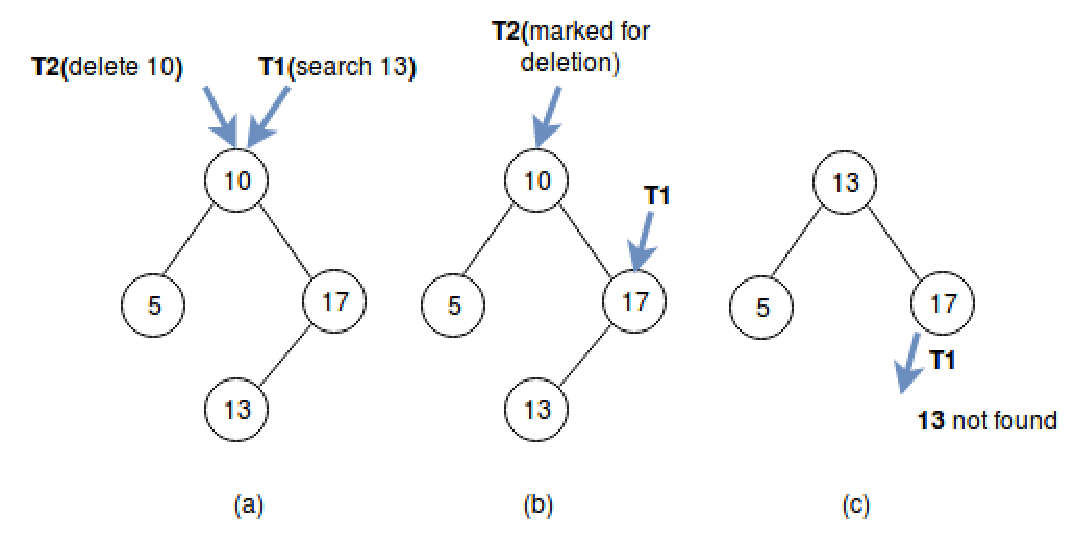
\includegraphics[width=11cm,height=5cm]{Concurrent_Search}
\caption{Concurrent Search with mutating operations. In (a) thread \textbf{T1} starts search for 13 whereas \textbf{T2} starts with searching for the node with key 10 for deletion. In (b), \textbf{T1} descends down and \textbf{T2} deletes 10 by replacing it with its successor 13 and deletes 13 physically from the tree. In (c), 13 is physically moved at root and \textbf{T1} fails}
\label{fig:concurrent_search}
\end{figure}

\section{Logical Ordering}
A binary search tree stores elements in such a way that a total order can be maintained between them. One such ordering can be obtained by \textit{inorder traversal} of the tree which results in non-decreasing ordering of elements. For instance, inorder traversal of the BST in Fig \ref{fig:concurrent_search}(a) results in \{5,10,13,17\}. To avoid edge cases, we add -$\infty$ and $\infty$ as smallest and largest elements present in the tree which yields the ordering \{-$\infty$, 5, 10, 13, 17, $\infty$\}. Logical ordering of tree-elements can be maintained by storing \textit{inorder-successor} and \textit{inorder-predecessor} information for each node. This enables accessing the next/previous element in the ordering layout through a single pointer instead of traversing several pointers along the physical layout of the tree. As logical ordering remains stable despite mutating operations, search operation can proceed concurrently with mutating operations. Maintaining ordering information results in space overhead but saves time while accessing successors or predecessors required by \textit{delete operation}. It also represents some time overhead as it requires updating the ordering information when it changes, but allows search operations to proceed without any synchronization over the tree layout. \\
\indent  To show how concurrent lock-free search operation can be performed, we consider the example in fig \ref{fig:concurrent_search}. Initial ordering of the tree elements is \{-$\infty$, 5, 10, 13, 17, $\infty$\}. After T2 deletes 10 from the tree, ordering is updated to \{-$\infty$, 5, 13, 17, $\infty$\}. Earlier when T1 was searching for 13, it failed to find 13 as it was moved to root due to concurrent deletion of 10. However with logical ordering in place, after T1 reaches at 17, as 13 < 17, it finds that the left child of 17 is NULL, it looks up the predecessor of 17 and finds that 13 is present in the tree and successfully terminates. 

\section{Concurrent Operations using Logical Ordering}
To maintain the logical ordering of the key elements of the tree, each node is extended with two pointers, \textbf{succ} and \textbf{pred} to store the address of the successor and the predecessor respectively. By using \textit{succ} pointer, successor of a node can be obtained following a single pointer which, otherwise, would require traversing the path from node to successor which could result in the thread being locked for a longer period of time due to concurrent updates on the path. From here onwards, we denote a node with key $k$ as $N_k$

\textbf{Updating \textit{succ} and \textit{pred} fields upon insert and delete}: When a node $N_k$ is inserted in the tree, it either becomes left or right child of its parent $p$. When it becomes left child of $p$, $p$ becomes it's successor, predecessor otherwise. When it is inserted to the left of $p$, following changes occur: 
\begin{itemize}
\item $p$.\textbf{pred}.\textbf{succ} = $N_k$
\item $N_k$.\textbf{succ} = p  
\item $N_k$.\textbf{pred} = p.\textbf{pred}
\item $p$.\textbf{pred}= $N_k$
\end{itemize}

following changes occur when $N_k$ is inserted to the right of p:
\begin{itemize}
\item p.\textbf{succ}.\textbf{pred} = $N_k$
\item $N_k$.\textbf{succ} = p.\textbf{succ}
\item $N_k$.\textbf{pred} = p
\item $p$.\textbf{succ} = $N_k$
\end{itemize}
 Fig \ref{fig:succ_pred_insert} shows the changes that occur after a node is inserted. 
\begin{figure}
\centering
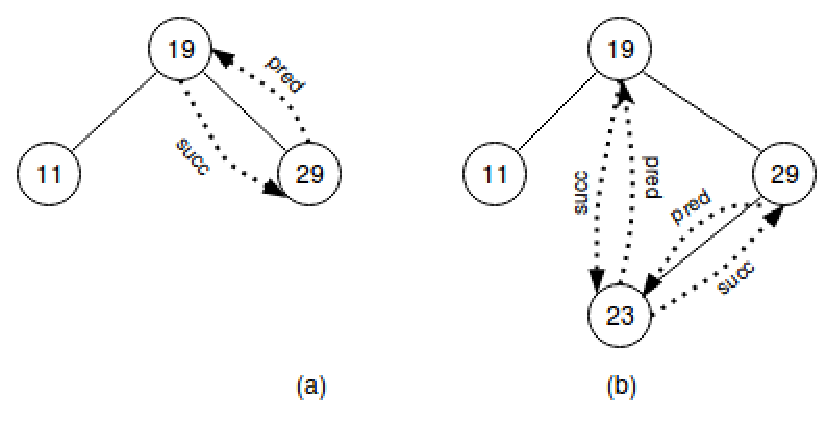
\includegraphics[width=9cm, height= 4cm]{succ_pred_insert}
\caption{Updating successor and predecessor pointer after an insert}
\label{fig:succ_pred_insert}
\end{figure}

\indent upon deletion, irrespective of the number of children the deleted node has, its successor and predecessor are set to point to each other.  

\section{Algorithm}
Node structure is modified to accommodate the additional fields incorporated for    correct operations in concurrent environment. Node contains \textit{mark} field to indicate if node is deleted; initially, it is set to \textbf{false}. Whereas \textit{tree\_lock} protects tree's physical layout fields, \textit{succ\_lock} protects tree's logical ordering fields, \textit{succ} and \textit{pred}. Initially, tree contains two nodes with keys -$\infty$ and $\infty$, both being predecessor and successor of each other. Node $N_{\infty}$ is made the root node and $N_{-\infty}$ the sentinel node which can only be accessed via \textit{pred} pointer in tree's logical ordering layout. 

\begin{lstlisting}[language=c++]
        struct Node<T>{
            T key;
            int height;
            struct Node<T> left,right;
            struct Node<T> parent;
            struct Node<T> succ,pred;
            Lock succ_lock, tree_lock;
            bool mark;                
        }
\end{lstlisting}

\subsection{Search} 
The \textit{search} operation is performed the same way as in sequential implementation. As \textit{Search} does not acquire locks on tree's physical layout fields and doesn't restart, it is oblivious to the location updates caused by other concurrent operations. Some elements, $k$, despite being present in the tree, may not be returned by \textit{search} due to mutating operations as shown in fig. \ref{fig:concurrent_search}. In such cases, we determine two nodes $N_{k1}$ and $N_{k2}$ in the tree such that $k \in (k1, k2)$. To find $N_{k1}$,    \textit{pred} pointers are traversed, starting from the node returned by \textit{search}, until a node with key $\leq k$ is found; similarly, $N_{k2}$ is obtained by traversing \textit{succ} pointers until a node with key $\geq k$ is found. Finally, k is compared with the key returned by traversing \textit{succ} pointers in the logical ordering layout of the tree and terminates successfully if equal, fails otherwise.

\begin{algorithm}
\caption{Search in concurrent environment}
\begin{algorithmic}[1]
\Function{Concurrent\_search}{$k$}:
\State node= search($k$);
\While{$k$ < node.key}
    \State node= node.pred;
    \EndWhile
\While{$k$ > node.key}
    \State node= node.succ
    \EndWhile 
\State \textbf{return} (node.key ==$k$ $\&\&$ !node.mark)
\EndFunction
\end{algorithmic}
\end{algorithm}

\subsection{Insert} 
\textit{Insert}($k$) operation starts with by calling \textbf{search}($k$) which returns a node $n$. If update operations don't modify $n$ after it was returned by search, $n$ can be a node with key $k$ or a node containing successor of $k$ or (iii) a node containing predecessor of $k$. Next, successor and predecessor of $k$ in the tree, namely \textbf{s} and \textbf{p}, are determined and \textbf{p} is locked using \textit{succ\_lock}. If $k \in$ (\textbf{p}, \textbf{s}] and \textbf{p} is not marked it moves to next step, otherwise operation restarts as update operations had modified the location of insert and \textbf{p} is unlocked. If \textbf{s} contains key equal to $k$ operations fails, releases lock on \textbf{p} and terminates; otherwise successful insertion begins by choosing the correct parent between \textbf{s} and \textbf{p} and locking it before updating the logical ordering followed by physical layout fields of the tree. Finally, rebalancing operation is applied, if required, to balance the imbalanced nodes. 

\begin{algorithm}
\caption{Concurrent Insert in AVL Trees}
\begin{algorithmic}[1]
\Function{concurrent\_insert}{$k$}
\While{$true$}
 \State   n = search($k$)
 \State   p = n.\textit{key} < $k$ ? n : n.\textit{pred}
 \State   lock(p.succ\_lock)
 \State   s = s.succ
 \If{k $\in$ (p.$key$, s.$key$] \&\& !p.$mark$}
    \If{s.\textit{key} $\geq$ $k$}
            \State unlock(p.succ\_lock)
            \State \textbf{return} \textit{false}
        \EndIf
    \State parent = choose\_parent(n,p,s)
    \State insert\_to\_tree($k$,parent,s,p)
    \State unlock(p.succ\_lock)
    \State grand\_parent = lock\_parent(parent)
    \State rebalance(grand\_parent,parent);
    \State \textbf{return} \textit{true}
 \EndIf
   \State unlock(p.succ\_lock)
\EndWhile
\EndFunction
\end{algorithmic}
\end{algorithm}

\begin{algorithm}
\caption{Updates logical and physical layout fields after insertion}
\label{alg:update}
\begin{algorithmic}[1]
\Function{insert\_to\_tree}{$k$, parent, s, p}
\State new\_node = create\_node($k$)
\State new\_node.parent = parent
\State new\_node.height = 0
\State new\_node.pred = p
\State new\_node.succ = s
\State p.succ = new\_node
\State s.pred = new\_node
\If{$k$ < parent.\textit{key}}
    \State parent.left = new\_node
\Else \State parent.right = new\_node
\EndIf
\State parent.height= \textbf{max}(parent.left.height, parent.right.height) + 1
\EndFunction
\end{algorithmic}
\end{algorithm}

\subsection{Choosing Correct Parent}
In sequential BST, the node returned by search operation is the actual parent, if its key is different than the key being inserted whereas the same may not hold in concurrent insertions. For example, in fig. \ref{fig:concurrent_insert}(a) , two threads \textbf{T1} and \textbf{T2} try to perform \textit{insert}(5) and \textit{insert}(9) concurrently where \textit{search}(5) and \textit{search}(9) return the same node $N_7$. After determining the predecessor and successors using returned node, \textbf{T1} acquires \textit{succ\_lock} on $N_{-\infty}$ and \textbf{T2} acquires \textit{succ\_lock} on $N_7$. Next, \textbf{T1} acquires \textit{tree\_lock} on $N_7$(and hence \textbf{T2} gets suspended) and $N_{11}$ and adds $N_5$ to the left of $N_7$ and observes that the balance factor at $N_{11}$ is violated hence performs single right rotation to balance the tree and releases the acquired locks to be acquired by \textbf{T2} which observes that $N_7$ can't be its parent anymore and chooses $N_{11}$ as its parent. It is guaranteed that either successor or predecessor would be chosen as parent once required tree\_locks are acquired which would prevent any concurrent rotation at the locked node. 

\begin{figure}
\centering
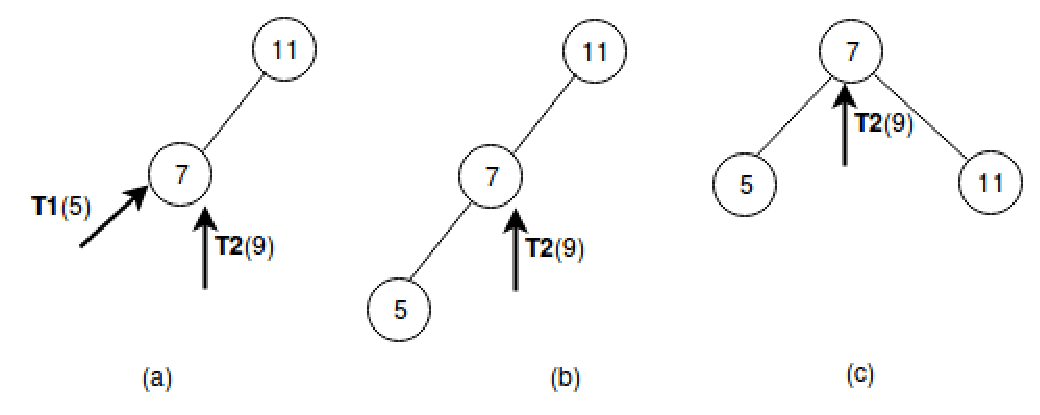
\includegraphics[width=10cm, height=4.5cm]{Concurrent_insert}
\caption{(a) Threads \textbf{T1} and \textbf{T2} try to acquire the tree\_lock on $N_7$ (b) \textbf{T1} succeeds and inserts 5 in the tree (c) \textbf{T2} observes that $N_7$ can't be its parent anymore}
\label{fig:concurrent_insert}
\end{figure}

\begin{algorithm}
\caption{Choosing the correct parent}
\begin{algorithmic}[1]
\Function{Choose\_Parent}{succ, pred, node}
\State parent = (node==pred || node == succ ? node: pred)
\While{true}
\State lock(parent.tree\_lock)
    \If{parent == pred}
        \If{parent.right == NULL} 
            \State \textbf{return} parent
        \EndIf
        \State unlock(parent.tree\_lock)
        \State parent = succ
    \Else 
        \If{parent.left == NULL}
            \State \textbf{return} parent
        \EndIf
        \State unlock(parent.tree\_lock)
        \State parent = pred
    \EndIf
\EndWhile
\EndFunction
\end{algorithmic}
\end{algorithm}

After choosing the correct parent, which is locked, physical and logical ordering layout fields are modified to bring about the changes after insertion as shown in algorithm \ref{alg:update}. Next, attempt is made to lock the parent of the parent, i.e. grandparent of $N_k$ and after acquiring the \textit{tree\_lock}, if grandparent node is marked, operation restarts otherwise it is chosen as the grandparent. Finally, rebalance operation is called on two locked nodes, i.e. parent and grandparent to update the heights of the nodes on the insertion path, if required, by performing appropriate rotations. 

\subsection{Delete Operation}
Delete operation proceeds in the same way as \textit{insert}. First, it calls search($k$), determines the predecessor($p$) of $k$ in the tree using the returned node, acquires the \textit{succ\_lock} on $p$ and applies the same validation as in insert. If validation succeeds, $k$ is locked via \textit{succ\_lock} and  required \textit{tree\_lock}s are acquired before marking the node to indicate that it was deleted from the tree. Next, logical ordering fields are updated by making $N_p$ and $N_k$.succ to point to each other, i.e. $N_p$ becomes predecessor of $N_k$.succ and $N_k$.succ becomes successor of $N_p$. Locks on $N_p$ and $N_k$ are released before updating physical layout fields of the tree. Physical deletion of the node $k$ happens the same way as in sequential operation except affected nodes in concurrent operations are locked before performing updates. Heights are updated through rebalance operations which starts from original parent of $N_k$.succ if $N_k$ had two children, $N_k$'s parent if it had less than two children or $N_k$.succ if $N_k$ was the parent of $N_k$.succ. 

\begin{algorithm}
\caption{Delete operation}
\label{alg:delete}
\begin{algorithmic}[1]
\Function{delete}{$k$}
\While{\textit{true}}
    \State n= search($k$)
    \State p= n.$key$ < $k$ ? n : n.\textit{pred}
    \State lock(p.succ\_lock)
    \State s= p.\textit{succ}
    \If{$k \in $(p.\textit{key}, s.\textit{key}] \&\& !p.mark}
        \If{s.\textit{key} > $k$}
            \State unlock(p.\textit{itsucc\_lock})
            \State \textbf{return} \textit{false}
        \EndIf
        \State lock(s.\textit{succ\_lock})
        \State has\_two\_children =acquire\_tree\_locks($s$)
        \State s.mark =\textit{true}
        \State s\_succ = s.\textit{succ}
        \State s\_succ.\textit{pred} = p
        \State p.\textit{succ} = s\_succ
        \State unlock(p.\textit{succ\_lock})
        \State unlock(s.\textit{succ\_lock})
        \State remove\_from\_tree(s,has\_two\_children)
        \State \textbf{return} \textit{true}
    \EndIf
    \State unlock(p.\textit{succ\_lock})
\EndWhile
\EndFunction
\end{algorithmic}
\end{algorithm}

\subsubsection{Acquiring Tree-locks}
Removal of nodes having two children is carried out differently than those with less than two as different number of locks need to be acquired. The process starts by acquiring the \textit{tree\_lock} on the node($n$) to be deleted followed by acquiring lock on its parent($p$). On success, it tries to acquire \textit{tree\_lock}s on
\begin{itemize}
\item $n$'s successor($s$), parent of $s$ and $s$'s child(if it exist) when $n$ has two children or
\item $n$'s child(if it exists) when $n$ has less than two chlidren
\end{itemize}

\begin{algorithm}
\caption{Acquire Necessary tree\_locks to delete the node}
\begin{algorithmic}[1]
\Function{acquire\_tree\_locks}{$n$}
\While{\textit{true}}
    \State lock(n.tree\_lock)
    \State r = n.\textit{right}
    \State l = n.\textit{left}
    \If{r == NULL || l==NULL}
        \If{r != NULL \&\& !try\_lock(r.\textit{tree\_lock})}
            \State unlock(node.\textit{tree\_lock})
            \State \textbf{continue}
        \ElsIf{l != NULL \&\& !try\_lock(l.\textit{tree\_lock})}
            \State unlock(node.tree\_lock)
            \State \textbf{continue}
        \EndIf
        \State \textbf{return} NULL
    \EndIf
    \State successor= $n$.succ
    \State parent =$n$.parent
    \If{parent != $n$}
        \If{!try\_lock(parent.\textit{tree\_lock})}
            \State unlock($n$.tree\_lock);
            \State \textbf{continue}
        \ElsIf{parent != successor.parent || parent.mark}
            \State unlock(parent.\textit{tree\_lock});
            \State unlock($n$.tree\_lock)
            \State \textbf{continue}
        \EndIf
    \EndIf
    \If{!try\_lock(successor.\textit{tree\_lock})}
        \State unlock($n$.tree\_lock)
        \If{parent !=$n$}
            \State unlock(parent.\textit{tree\_lock})
        \EndIf
        \State \textbf{continue}
    \EndIf
    
    \State succ\_right = successor.\textit{right}
    \If{succ\_right != NULL \&\& !try\_lock(succ\_right.\textit{tree\_lock})}
        \State unlock($n$.tree\_lock)
        \State unlock(successor.tree\_lock)
        \If{parent != $n$}
            \State unlock(parent.tree\_lock)
        \EndIf
        \State \textbf{continue}
    \EndIf
    \State \textbf{return} successor
\EndWhile
\EndFunction
\end{algorithmic}
\end{algorithm}

If process fails to acquire lock on any of the nodes, it releases the acquired locks on other nodes and operations restarts from trying to acquire locks on $n$ and its parent. It is necessary to check the number of children n has in each iteration as the number of children $n$ has, may change due to concurrent updates from other threads. Operation terminates after successfully acquiring all the required locks. Physical removal of the node is performed the same as in sequential implementation.  


\subsection{Rebalancing}
Update operations in AVL trees may create imbalance at certain nodes. One of four types of rotations are applied to balance the imbalanced nodes. Rebalancing process starts from the location of update and moves up till the root applying rotations, wherever required, to balance the tree. After insertion, it starts from the parent(p) and grandparent(g) of the inserted node; after deletion, it starts from the parent(g) of the deleted node and its child(p) if the node had less than two children(could be null if none) otherwise parent(g) and left-child(maybe null)(p) of the successor of the deleted node. During upward traversal of the tree, the rebalance operation locks \textit{g} and \textit{p} first to update their heights. Operation terminate if height of \textit{g} does not change and height invariant property at \textit{g} is not violated, it continues upwards by updating \textit{p} to \textit{g} and \textit{g} to its parent if height of \textit{g} changes and balance factor remains valid, rotation takes place otherwise. When balance factor at \textit{g} is not valid and height of the
subtree containing \textit{p} is smaller than the other subtree, \textit{p} is unlocked and attempt to acquire the lock on the other child of \textit{g} is made. If attempt succeeds, \textit{p} is made to point to the other child of \textit{g}, otherwise all currently locked nodes are unlocked and attempt to acquire the locks on them restarts. If \textit{g} is marked i.e. deleted, operation terminates. 


 %%%%%%%%%%%%%%%%%%%%%%%%%%%%%%%%%%%%%%%%%%%%%%%%%%%%%%%%%%%%
% Appendices.

\chapter{Overview of Cuda Architecture}
\label{chap:cuda}
Widespread demand for improving performance of consumer and industrial computing devices resulted in evolution of high-speed processors. However, due to various fundamental limitations in the fabrication of the integrated circuits, restrictions in heat and power consumption and limit in the size of transistors, it is no longer feasible to increase the CPU clock-speed in order to extract more powerful computation from existing architecture. \\
\indent Graphics processing units(GPUs) were created to satisfy market demand for high speed realtime graphics processing. Since then it has evolved into highly parallel, multithreaded, manycore processor with tremendous computational horsepower and very high memory bandwidth. Since GPUs are designed for highly parallel and compute intensive applications, more transistors are devoted to data processing rather than data caching and flow control. 
   

\section{Why GPU computing?} GPUs are designed to solve problems which show data-parallelism, i.e. same set of instructions execute on multiple data elements in parallel where operations on data involve more arithmetic computations than memory accesses. Since same set of instruction execute for each data element, control flow instructions are used quite less and as operations require intense arithmetic computations as compared to memory accesses, memory access latency can be hidden by greater arithmetic calculations instead of designing big and efficient data caches.\\
\indent Generally CPUs contain just few cores which come with their own private and shared caches and process just 10s of software threads concurrently whereas a GPUs consist of hundreds of cores that can handle thousands of threads simultaneously. These capabilities enable GPUs to execute data-parallel task several times faster than CPU cores. Whereas GPUs provide execution speedup by diving task among thousands of threads, they are cost and power efficient as compared to CPUs.

\section{Cuda}

\textbf{CUDA}(\textit{Compute Unified Device Architecture}) is a parallel computing platform which provides APIs to harness compute capability of NVIDIA GPUs. It provides libraries that enable data transfer between host and devices where host refers to CPU and its memory and  device refers to GPUs and their memory. A typical sequence of operations during execution of cuda programs are:
\begin{itemize}
\item Declare and allocate memory on host and device
\item Initialize host elements
\item Copy host data to device memory
\item Launch the kernels and perform computation
\item Copy data back from device memory to host memory
\end{itemize}

 
CUDA organizes threads into hierarchy of \textit{warps}, \textit{blocks} and \textit{ grids}. It incorporates \textit{global memory} concept which is shared by all the threads of the grid and \textit{shared memory} which is shared by threads of a block. In order to ensure correctness of computation and avoid race conditions and deadlock, it provides \textit{synchronization} primitives. The hierarchy in the thread organization helps programmers break their task into smaller and parallelizable tasks that can be executed independently by a warp/block of threads. CUDA runtime system manages execution of threads by launching thread blocks on available streaming multiprocessors(SM) and thereby relieving programmers from tedious task of thread management.

\subsection{Programming Model}
\subsubsection{Kernels} CUDA kernels are the entry point for execution of programs on GPU cores. Kernels have the similar syntax as C functions but when invoked execute as many number of times as the number of threads launched and all concurrently. Unlike C functions, CUDA kernels have only \textit{void} return type and their definition is preceded by  \textit{\_\_global\_\_} declaration specifier.  

\begin{lstlisting}[language=C++]
    __global__ void kernel(param1, param2,...){
        statements;
    }
\end{lstlisting}

CUDA kernels are invoked the same way as the functions in C except the kernel launch requires the number of threads to be specified that would execute it, which is specified within $<<<....>>>$.
\begin{lstlisting}[language=c++]
        kernel<<<t_x,t_y,t_z>>>(param1,param2,...);
\end{lstlisting}
 
Depending on the values of kernel launch parameters within $<<<...>>>$, a 3D/2D/1D grid of threads would be launched and each thread is assigned a unique id which can be used to control the execution of threads. 

\subsubsection{Thread Hierarchy}
Cuda organizes threads into 1-dimensional, 2-dimensional or 3-dimensional blocks of threads. Blocks are organized into 1-dimensional, 2-dimensional or 3-dimensional grid of blocks as illustrated in Fig. \ref{fig:thread_block_grid}. Threads within a block are indexed using \textbf{threadIdx} construct and blocks in a grid are indexed using \textbf{blockIdx}. Block and grid dimensions are accessed using \textbf{blockDim} and \textbf{gridDim} respectively. All the indexing and dimension constructs are three-field, namely x, y and z, structures. Local Id of a thread in a 3-dimensional block is calculated as:
\begin{lstlisting}
    local_threadId = blockDim.x * blockDim.y * threadIdx.z + blockDim.x * threadIdx.y + threadIdx.x
\end{lstlisting}
Similarly, block Id in a 3D grid is calculated as:
\begin{lstlisting}
    blockId = gridDim.x * gridDim.y * blockIdx.z + gridDim.x * blockIdx.y + blockIdx.x
\end{lstlisting}
and global Id of a thread is calculated as: 
\begin{lstlisting}
    global_threadId = blockId * (blockDim.x * blockDim.y * blockDim.z) + local_threadId
\end{lstlisting}

\begin{figure}
    \centering
    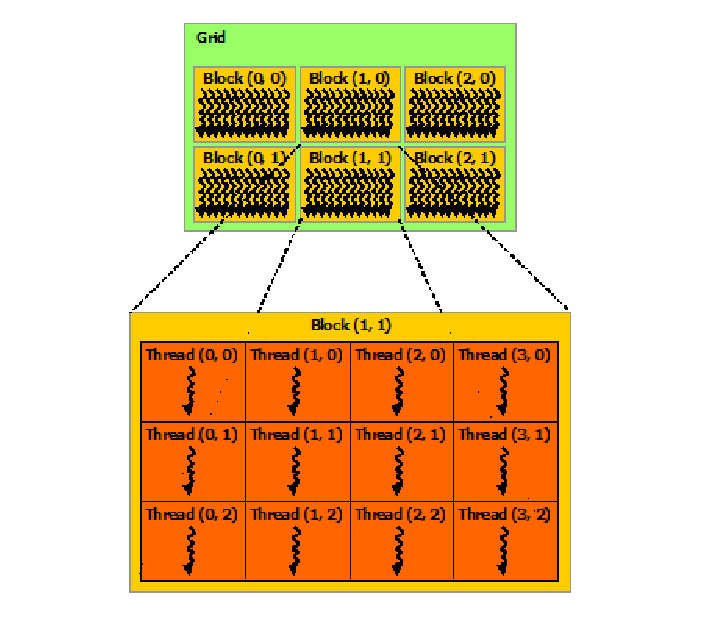
\includegraphics[width=12cm, height=8cm]{grid_of_thread_blocks}
    \caption{Organization of threads in grid and blocks}
    \label{fig:thread_block_grid}
\end{figure}

Due to hardware limitations, the number of threads per block and blocks per dimension of the grid are restricted. Thread blocks execute independently. However, they can be made to execute in some specified order by using atomics and locks.
Threads within a block can cooperate to perform some computations through shared memory. To coordinate memory accesses in such computations, threads are synchronized by calling \textit{\_\_syncthreads()} library function which acts as a barrier for the threads of each block. 

\section{Memory Hierarchy}
Cuda organizes  read and write memory into \textit{global}, \textit{shared} and \textit{private} types. Global memory can be accessed by all the threads executing across all the cores. Shared memory is per black and can only be accessed by threads executing within the block. Local or private memory is thread specific and can only be modified by the thread it was allocated for as shown in fig. \ref{fig:memory_hierarchy} Cuda also provides \textit{constant} and \textit{texture} memory spaces which are read-only and can be accessed by all the threads.  

\begin{figure}
\centering
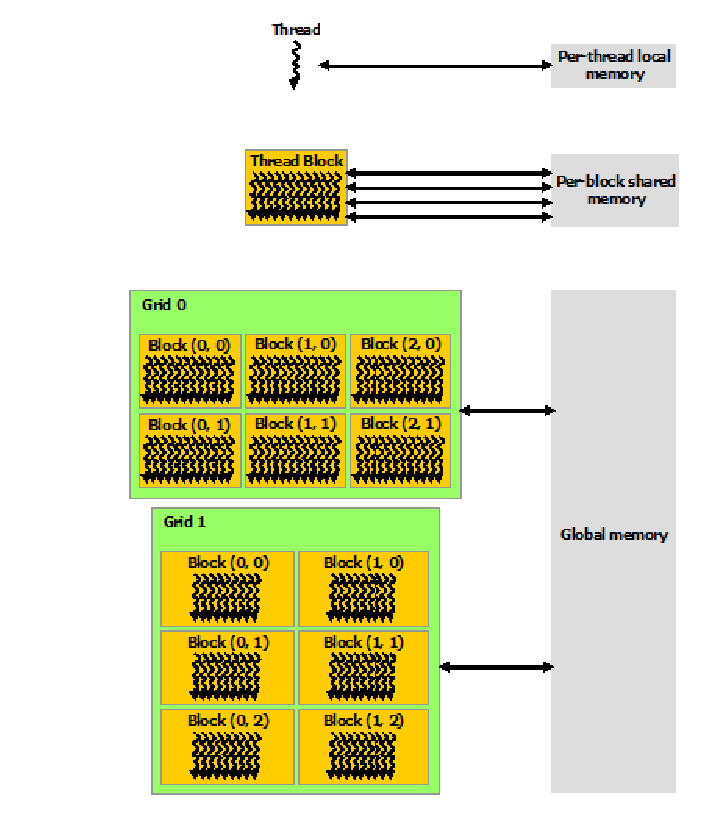
\includegraphics[width= 12cm, height= 11cm]{memory_hierarchy}
\caption{Device memory hierarchy}
\label{fig:memory_hierarchy}
\end{figure}

\chapter{Evaluation and Results}
\label{chap:results}
\section{Dataset}
Results were obtained by first inserting 1 million elements, created uniformly at random from the range (-$10^{8}$,$10^{8}$), in the tree. 
Before each test, test-data is generated uniformly at random from the range (-8N,8N) where N is the size of the dataset. Balanced Binary Search Trees are preferred over other data structures to store the data for their efficient search results. Therefore, in each test, number of search queries are in excess to the number of inserts and deletes. Test-data size ranges from 100 to 10 million and percentage of search, insert and delete queries in each dataset is kept as following:
\begin{itemize}
\item \textbf{type 1}: 100\% search, 0\% insert and 0\% delete
\item \textbf{type 2:} 50\% search, 50\% insert and 0\% delete
\item \textbf{type 3:} 50\% search, 0\% insert and 50\% delete
\item \textbf{type 4:} 50\% search, 25\% insert and 25\% delete
\end{itemize}

\section{Evaluation}
 Sequential and and concurrent cpu implementations were run on Intel i5-3210M processors with for processors and each consisting of 2 cores and operating at 2.50GHz. Concurrent cuda-implementation was run on NVIDIA's Tesla M2070 GPU cores.
 Performance is evaluated by comparing the times taken by all the threads to finish the execution of the operations assigned to them. Concurrent cpu implementation was tested by creating 128 threads for all sizes of the test data whereas concurrent gpu implementation was tested by creating as many number of threads as the number of queries when size of the test-data is less than 100000, 100000 otherwise. For each test-data size and mixture of query types, programs were run 10 times and time was taken as the average of all the execution. Following are the tabular and graphical representation of the results.
 
 \section{Observations}
When all the queries are search type, GPU implementation performs > 1000 times faster than the other implementations for all sizes of the test data. GPU implementation is faster because each GPU thread has to execute < 100 queries as compared to $\approx$ 10000 queries executed by concurrent CPU threads.

\begin{table}[H]
\captionof{table}{Test data consisting of 100\% search, 0\% insert and 0\% delete queries}
\begin{tabular}{|l|l|l|l|}
\hline
\textbf{Data set size} & \textbf{\begin{tabular}[c]{@{}l@{}}Sequential Execution\\ time(ms)\end{tabular}} & \textbf{\begin{tabular}[c]{@{}l@{}}Concurrent GPU\\  time(ms)\end{tabular}} & \textbf{\begin{tabular}[c]{@{}l@{}}Concurrent \\ CPU time(ms)\end{tabular}} \\ \hline

100                    & 0.0257406                                                                        & 0.000066                                                                    & 2.6127337                                                                   \\
1000                   & 0.262193                                                                         & 0.000075                                                                    & 3.704370                                                                    \\
10000                  & 2.84989                                                                          & 0.000161                                                                    & 4.5367625                                                                   \\
100000                 & 34.435                                                                           & 0.001249                                                                    & 12.8423605                                                                  \\
1000000                & 504.223                                                                          & 0.020151                                                                    & 54.135625                                                                   \\
10000000               & 6760.34                                                                          & 0.285816                                                                    & 176.508964  \\
\hline
\end{tabular}
\end{table}

\begin{figure}[H]
\centering 
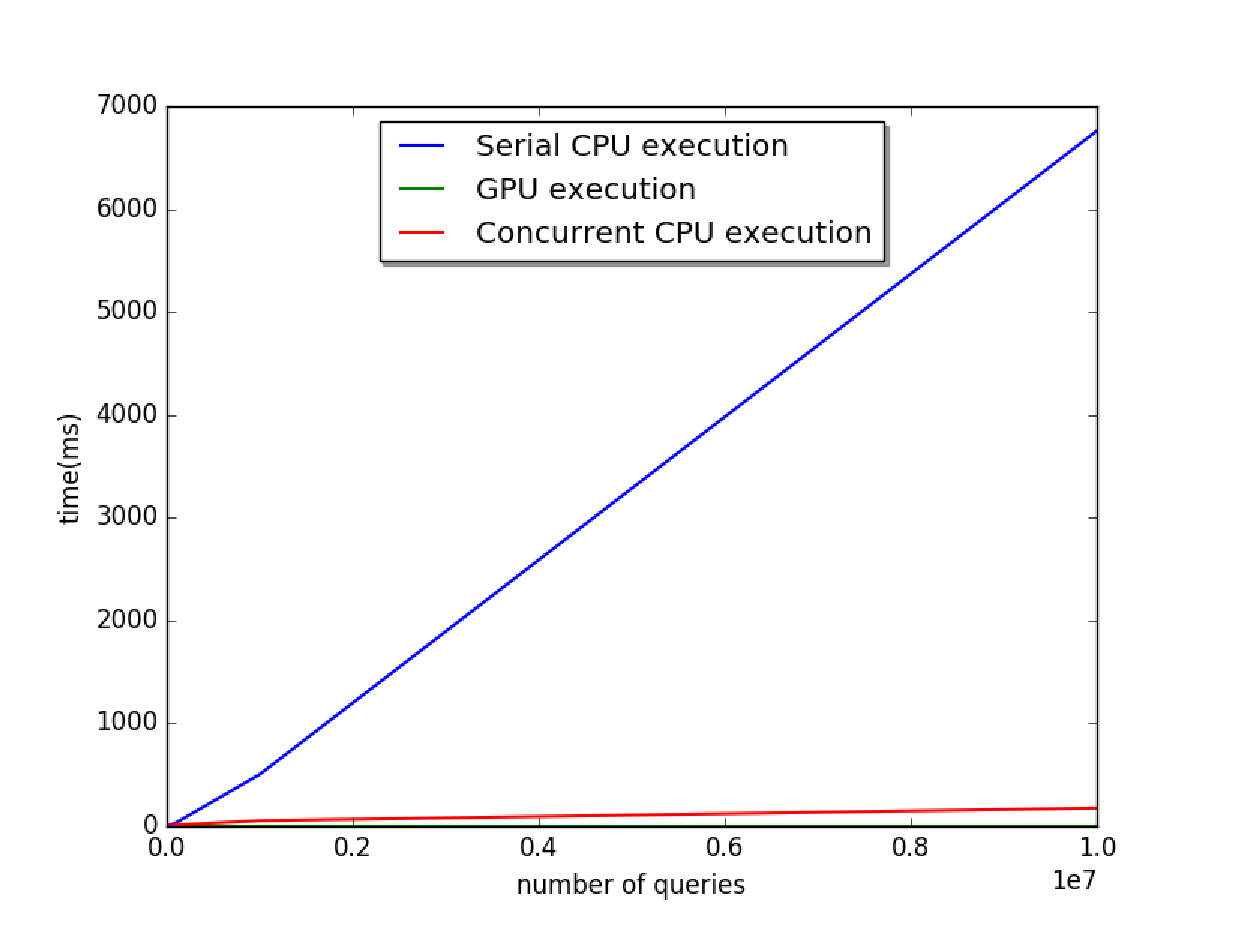
\includegraphics[width=13cm,height=10cm]{s_i_d_100_0_0}
\caption{100\% search query. Integers used as keys}
\label{fig:sid_100_0_0}
\end{figure}

When mix of search, insert and delete operations are used, Concurrent CPU implementation catches up with GPU implementation owing to use of locks in for the mutation operations 
\begin{table}[H]
\begin{tabular}{|l|l|l|l|}
\hline
\textbf{Data set size} & \textbf{\begin{tabular}[c]{@{}l@{}}Sequential Execution\\ time(ms)\end{tabular}} & \textbf{\begin{tabular}[c]{@{}l@{}}Concurrent GPU\\  time(ms)\end{tabular}} & \textbf{\begin{tabular}[c]{@{}l@{}}Concurrent \\ CPU time(ms)\end{tabular}} \\ \hline
100                    & 0.0604874                                                                        & 0.002042                                                                    & 3.4113046                                                                   \\
1000                   & 0.570185                                                                         & 0.021852                                                                    & 4.3562131                                                                   \\
10000                  & 6.02478                                                                          & 0.237240                                                                    & 8.2393948                                                                   \\
100000                 & 66.4861                                                                          & 2.442558                                                                    & 19.189123                                                                   \\
1000000                & 874.748                                                                          & 25.450551                                                                   & 103.853393                                                                  \\
10000000               & 11288.4                                                                          & 259.275844                                                                  & \textgreater30 mins \\  \hline                                                                
\end{tabular}
\caption{\label{tab:s_i_d_50_25_25} test data consisting of 50\% search, 25\% insert and 25\% delete}
\end{table}

\begin{figure}[H]
\centering 
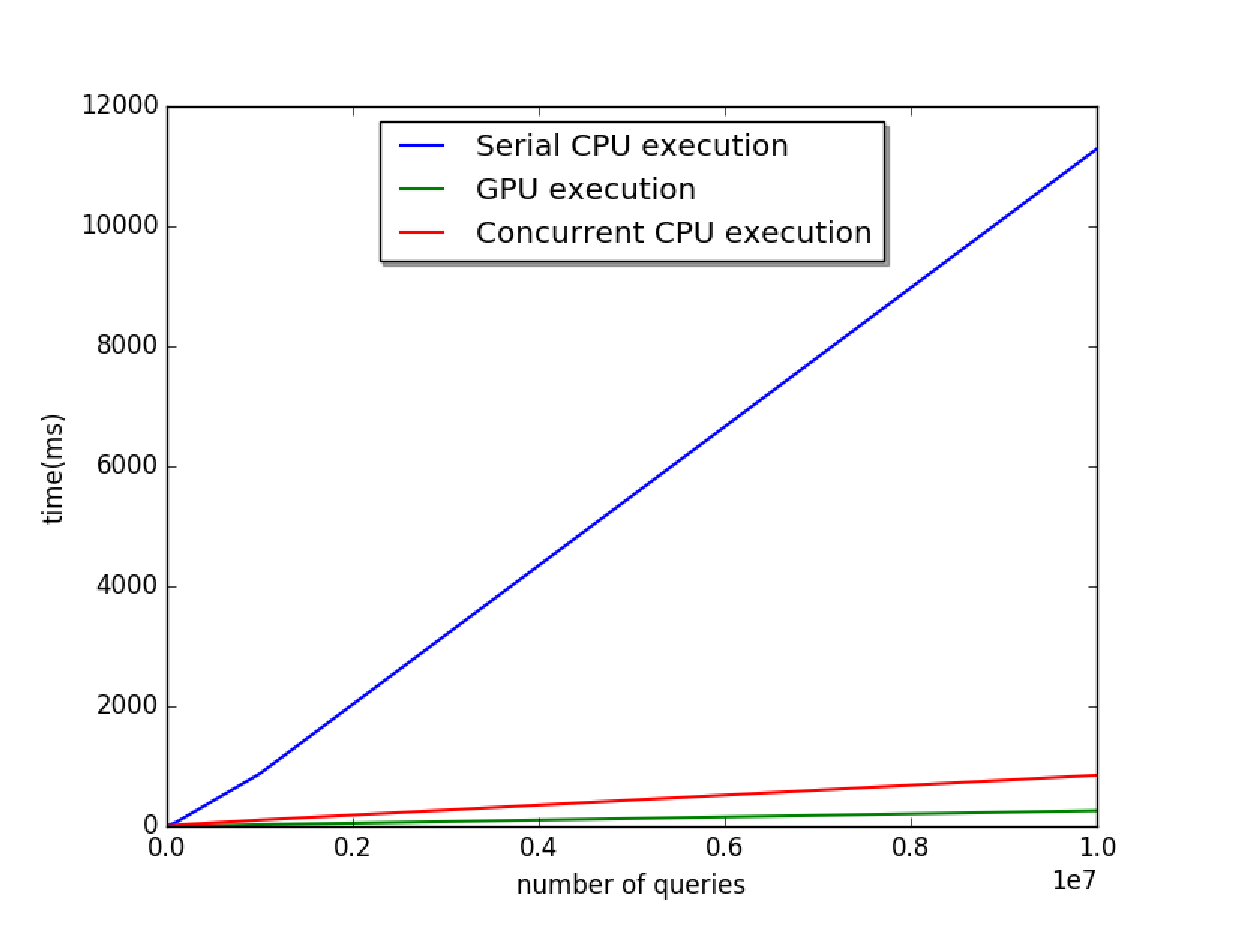
\includegraphics[width=13cm,height=10cm]{s_i_d_50_25_25}
\caption{50\% search, 25\% insert and 25\% delete query 0\%}
\label{fig:sid_50_25_25}
\end{figure}
When percentage of insert and delete operations is increased, CPU implementation catches up with the GPU implementation for large datasets, but fails to produce result within 30 mins for 10 million size dataset. Comparable performance of both the implementations can be attributed to the use of extensive locks in concurrent CPU implementation which makes the operations almost sequential as contention among threads increases with large number of queries resulting in threads taking up huge amount of to time to acquire the locks, as compared to GPU implementation which performs searches(which constitute 50\% of the queries) concurrently with inserts and deletes which are serialized to avoid the extensive use of locks which result in degraded performance.       
\begin{table}[H]
\begin{tabular}{|l|l|l|l|}
\hline
\textbf{Data set size} & \textbf{\begin{tabular}[c]{@{}l@{}}Sequential Execution\\ time(ms)\end{tabular}} & \textbf{\begin{tabular}[c]{@{}l@{}}Concurrent GPU\\  time(ms)\end{tabular}} & \textbf{\begin{tabular}[c]{@{}l@{}}Concurrent \\ CPU time(ms)\end{tabular}} \\ \hline
100                    & 0.0689402                                                                        & 0.002686                                                                    & 25.7077709                                                                  \\
1000                   & 0.677887                                                                         & 0.026318                                                                    & 32.625123                                                                   \\
10000                  & 7.35961                                                                          & 0.291068                                                                    & 47.826260                                                                   \\
100000                 & 77.9338                                                                          & 2.000197                                                                    & 59.2328736                                                                  \\
1000000                & 1071.12                                                                          & 21.630555                                                                   & 972.607328                                                                  \\
10000000               & 13826.7                                                                          & 232.478219                                                                  & \textgreater30 mins  \\ \hline                                                        
\end{tabular}
\caption{\label{tab:insert_50}test data consisting of 50\% search, 50\% insert and 0\% delete queries}
\end{table}


\begin{figure}[H]
\centering 
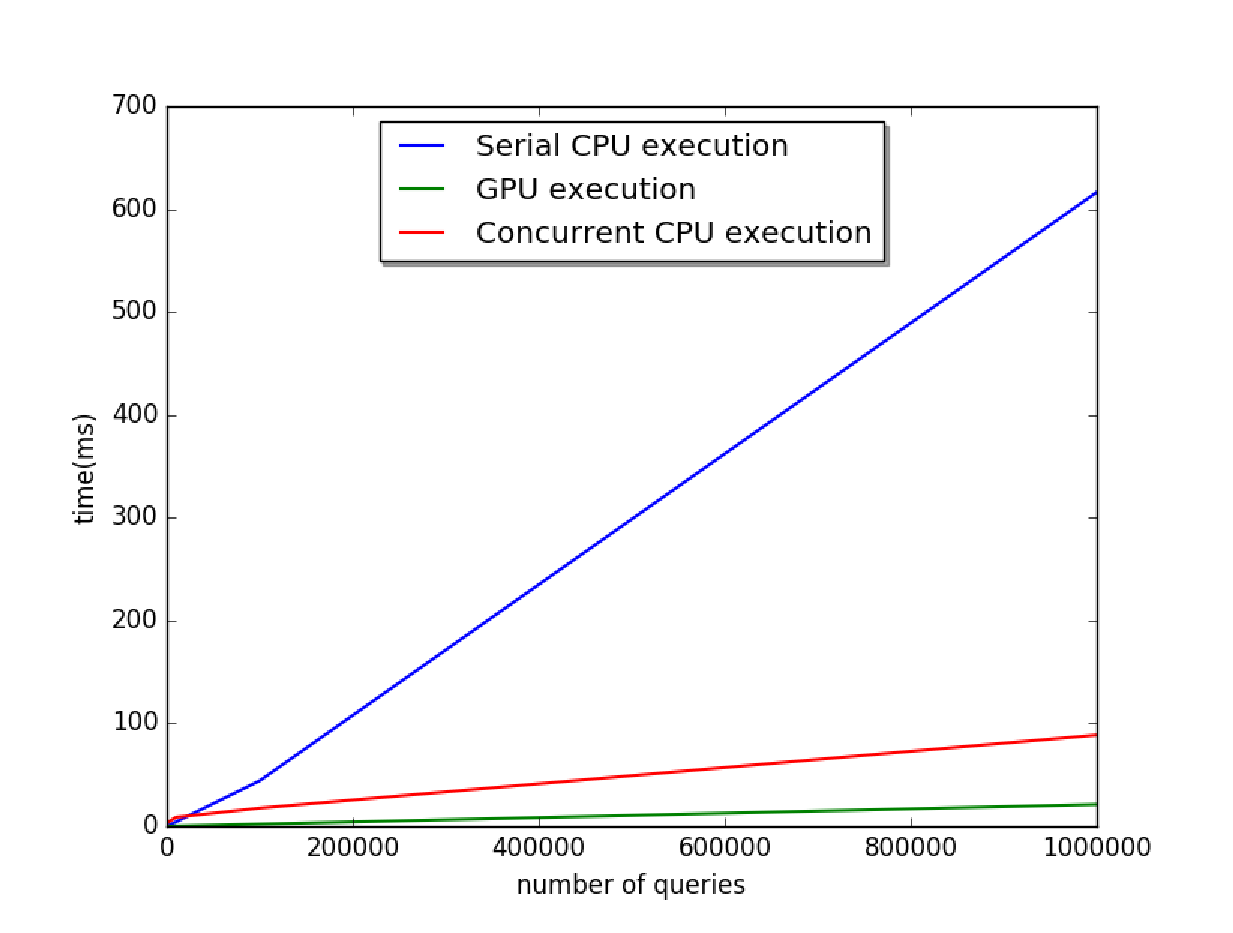
\includegraphics[width=13cm,height=10cm]{s_i_d_50_0_50}
\caption{50\% search and 50\% delete queries}
\label{fig:sid_50_0_50}
\end{figure}


\begin{table}[H]
\begin{tabular}{|l|l|l|l|}
\hline
\textbf{Data set size} & \textbf{\begin{tabular}[c]{@{}l@{}}Sequential Execution\\ time(ms)\end{tabular}} & \textbf{\begin{tabular}[c]{@{}l@{}}Concurrent GPU\\  time(ms)\end{tabular}} & \textbf{\begin{tabular}[c]{@{}l@{}}Concurrent \\ CPU time(ms)\end{tabular}} \\
100                    & 0.0347251                                                                        & 0.000979                                                                    & 2.7682338                                                                   \\
1000                   & 0.36965                                                                          & 0.018600                                                                    & 3.65853025                                                                  \\
10000                  & 4.26217                                                                          & 0.197995                                                                    & 8.765159                                                                    \\
100000                 & 4.2681                                                                           & 2.054536                                                                    & 17.6363476                                                                  \\
1000000                & 616.389                                                                          & 21.172125                                                                   & 88.64886775                                                                 \\
10000000               & 7219.87                                                                          & 203.620203                                                                  & \textgreater 30mins  \\ \hline                                                        
\end{tabular}
\caption{\label{tab:s_i_d_50_0_50}}
\end{table}

\begin{figure}[H]
\centering 
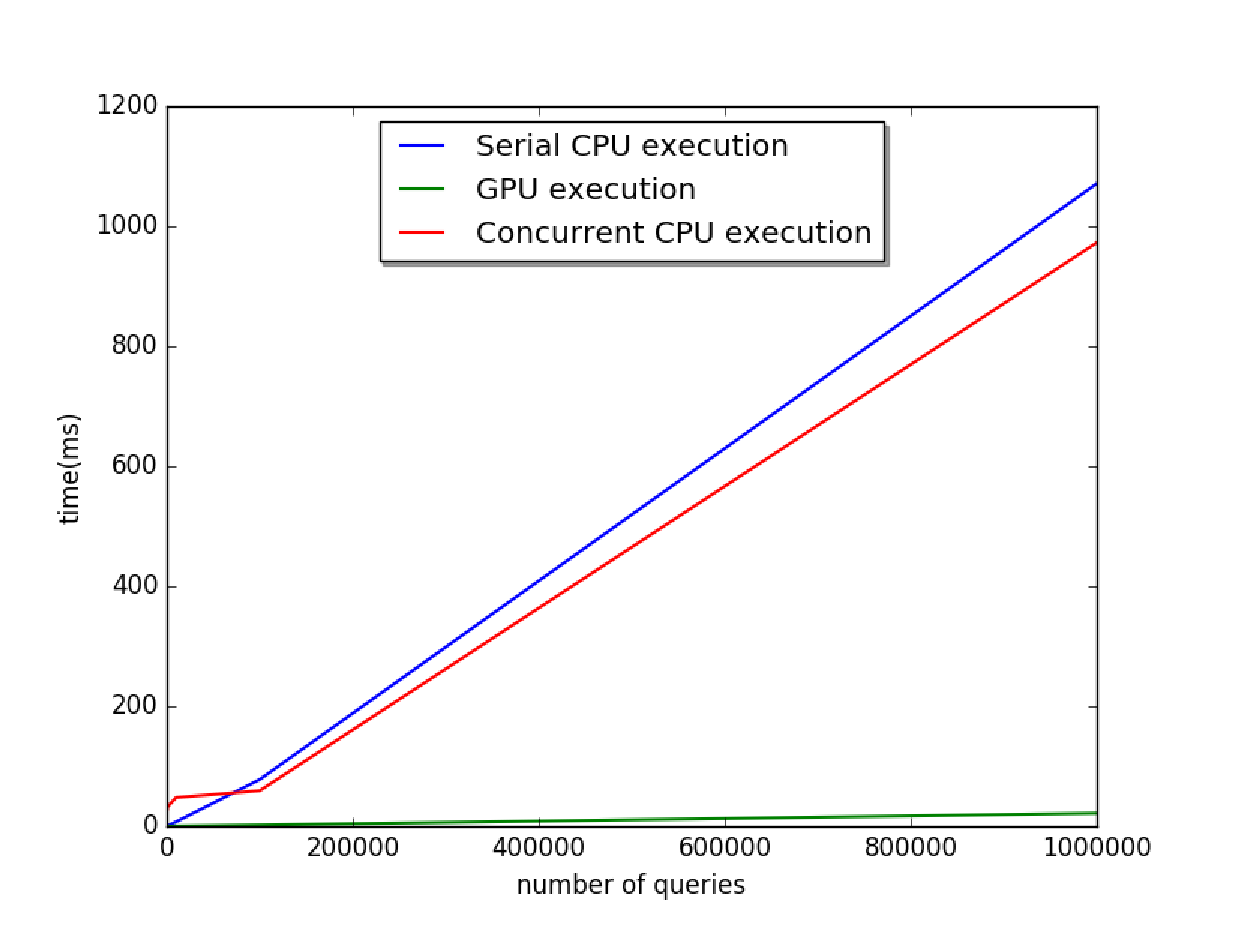
\includegraphics[width=13cm,height=10cm]{s_i_d_50_50_0}
\caption{50\% search and 50\% insert queries}
\label{fig:sid_50_50_0}
\end{figure}


\chapter{Future Work}
\label{chap:future_work}
Mutating operations are the bottleneck in the performance of algorithms on AVL trees. Locks are not advisable to be used on GPUs as they serialize the operations of the critical section they are used for. State of the art algorithms are designed to be run on CPUs but algorithms to to perform operations on AVL tree on GPUs have not been studied much. As parallel programming is becoming the requirement of almost all the applications for scalability and efficiency reasons, focus must be given on designing algorithms to perform lock-free operations on AVL tree as it is an excellent data structure to store the data and perform efficient search queries. Update operations, in AVL trees, require locking every node in the path while traversing up the tree, they become sequential when the number of queries increases. Balance factor constraint can be relaxed to mitigate the use of locks during concurrent operations. Logical Ordering of the tree elements allows concurrent lock-free search operations along with mutating operations. Similar approaches can be designed for insert and delete operations where certain number of insert or delete operations can be performed in some part of the tree like standard BST operations followed by rebalancing process for that part of the tree. Since much of the locking happen due to upward traversal of the operation upto root to rebalance the tree, constraints can be created to restrict the length of the path an operation would cover.

\chapter{Conclusion}
\label{chap:conclusion}
The main focus of the implementation was to improve the performance of the search queries in concurrent environment on GPUs while performing other operations concurrently, which was achieved by implementing the Logical Ordering of the tree elements that is explicitly maintained in the tree and separates look-up operations from those that update the layout of the tree. Logical ordering enables efficient lock-free lookup operations along with other mutating operations in the tree. Extensive use of locks degrades performance and hence limits the amount of concurrency that can be extracted from AVL tree operations. For the aforementioned reasons and AVL tree being the height balanced binary search tree allowing $\log(n)$ search operations, it preferred over other trees in applications that require large number of search queries and very less number of insert and removals to be performed on the stored data. GPUs scale well when operations are lock-free but don't show much better performance when locks are used.   


\begin{thebibliography}{1}

\bibitem{Parallel_Dictionaries}
Mulralidhar Medidi and Narsingh Deo. \emph{Parallel Dictionaries Using AVL Trees}. JOURNAL OF PARALLEL AND DISTRIBUTED COMPUTING 49, 146-155 (1998) ARTICLE NO. PC981432
\bibitem{ExpandedAVL}
Zhang Yin and Xu Zhuoqun. \emph{Concurrent Manipulation of Expanded AVL Trees}[J].  Journal of Computer Science and Technology, 1998,V13(4): 325-336
\bibitem{Unified_Approach}
Joaquim Gabarr\'o and Xavier Messeguer. \emph{A Unified Approach to Concurrent and Parallel Algorithms on Balanced Data Structures}.  Computer Science Society, 1997. Proceedings., XVII International Conference of the Chilean

\bibitem{Brother_Trees}
Joaquim Gabarr\'o and Xavier Messeguer.\textit{Parallel Dictionaries with Local Rules on AVL and Brother Trees}. ACM Journal on Information Processing Letters archive Volume 68 Issue 2, Oct. 30, 1998 
\bibitem{Ellis}
CARLA SCHLATTER ELLIS, \emph{Concurrent Search and Insertion in AVL Trees}. IEEE Transactions on Computers, September 1980  

\bibitem{PracticalConcurrent}
Nathan G. Bronson, Jared Casper. Hassan Chafi, Kunle Olukotun\textit{A Practical Concurrent Binary Search Tree}. \textit{PPoPP '10} Proceedings of the $15^th$ ACM SIGPLAN Symposium on Principles and Practice of Parallel Programming

\bibitem{Logical_Ordering}
Dana Drachsler, Martin Vechev. Eran Yahav; \textit{Practical Concurrent Binary Search Trees via Logical Ordering}. PPoPP '14 Proceedings of the $19^{th}$ ACM SIGPLAN symposium on Principles and practice of parallel programming 

\bibitem{Cuda Documentation}
Cuda C Programming Guide \url{http://docs.nvidia.com/cuda/cuda-c-programming-guide/}

\bibitem{Cuda by Example}
Jason Sanders, Edward Kandrot;\textit{Cuda By Example, An Introduction to General Purpose GPU Programming}

\bibitem{Massively Parallel}
David B. Kirk and Wen-mei W. Hwu; \textit{Programming Massively Parallel Processors, A Hands-on Approach}

\end{thebibliography} 
\end{document}